%===============================================================================
% $Id: ifacconf.tex 19 2011-10-27 09:32:13Z jpuente $  
% Template for IFAC meeting papers
% Copyright (c) 2007-2008 International Federation of Automatic Control
%===============================================================================
\documentclass{ifacconf}

\usepackage{graphicx}      % include this line if your document contains figures
\usepackage{natbib}        % required for bibliography
\usepackage{amsmath}
\usepackage{amssymb}
\usepackage{epstopdf}
\usepackage{algorithm,algorithmic}

%===============================================================================
\def\ve#1{\mathchoice{\mbox{\boldmath$\displaystyle#1$}}
{\mbox{\boldmath$\textstyle#1$}}
{\mbox{\boldmath$\scriptstyle#1$}}
{\mbox{\boldmath$\scriptscriptstyle#1$}}} 

\newcommand{\dd}{\text{d}}
\newcommand{\dt}{\dd t}
\newcommand{\ff}{\text f}
\newcommand{\eg}{\text{e.g., }}
\newcommand{\ie}{\text{i.e., }}
\newcommand{\wrt}{\text{w.r.t. }}
\newcommand{\ww}{\text w}
\newcommand{\st}{\text{s.t.}}
\newcommand{\mx}{\text{max}}
%\newtheorem{defn}[thm]{Definition}
%
\begin{document}
\begin{frontmatter}

\title{Parallelotopes.An alternative for Robust MPC.}
%Different Recursive Optimal Parallelotopic Outbounding(ROPO) algorithms in Robust Control 
% Parallelotopes on Robust Control???.

\thanks[footnoteinfo]{Sponsor and financial support acknowledgment
goes here. Paper titles should be written in uppercase and lowercase
letters, not all uppercase.}

\author[First]{Carlos E. Valero} 
\author[First]{Radoslav Paulen} 

\address[First]{Slovak University of Technology in Bratislava, Slovakia,
(e-mail: \{carlos.valero, radoslav.paulen\}@stuba.sk).}

\begin{abstract}                % Abstract of not more than 250 words.
In this paper the problem of Robust Model Predictive Control (RMPC) using parallelotopes is considered. Firstly, it was developed two common approaches of Recursive Optimal Parallelotopic Outbounding(ROPO). Follows by the design of two efficient algorithm able to enhance the previous methodologies with respect to objective function of the MPC. All methodologies are tested using a double integrator. It is assumed any kind of distribution in the noise of the output, but always with a known bounded. The results obtained proof the validity of these new methods and a robustness against constrain on the states. 
\end{abstract}

\begin{keyword}
Predictive control, Robustness, Optimization problems, Bounded noise, Uncertainty, System state estimation

\end{keyword}

\end{frontmatter}
%===============================================================================

\section{Introduction}
Nowadays, the industries tackle the robustness in their processes to avoid losses and to guarantee optimal production. Robustness is an important concept used in control theory for establishing insensitive to noise variation. The robustness is reached after guaranteeing that the plant runs under its constraints even for undesired noises. One of the way to approaches this is by considering two different processes inside. The identification and control processes. The control process is extremely relate to the identification. Therefore, identify the states of a systems is an invaluable task. A good identification process will avoid any constraint violation and enhance the performance of the system. However, this job is difficult, usually because of inaccuracy of the plant model taken, and the presence of noise that, although, it is bounded in several systems for physical restrictions, it can have different and complex distributions. On the other hand, after selecting an identification process. The control section must deal with many varieties of constraints to guarantee a robust yield \citep{maciejowski2002}. In this work, it is presented a linear model predictive control (MPC),together to a Recursive Optimal Parallelotopic Outbounding (ROPO) algorithm as an identification system what it will guarantee robustness in all states of the plant.

Due to the importance of the identification process, there are many developments in this area. The range of works starts with the simplest such as the well known Luenberger estimator that does not take into account optimality or uncertainties, \citep{dorf2011modern}, \citep{Zonotopes_text}. It is followed by the Kalman Filter also known as linear quadratic estimation (LQE), is an algorithm that uses statistical noise, and produces estimates of the states variables that tend to be more accurate than Luenberger estimator. More modern   estimator could lies on the use of intelligent techniques such as neural networks, fuzzy logic, genetics algorithms and so on; or on estimators using some type of polyhedron form like polytopes, zonotopes \citep{Comb2003},\citep{sco14},\citep{Zonotopes_text} ellipsoids, \citep{Filippova1996}, \citep{kur97} or like the case of this paper, a special type of zonotope called parallelotope, \citep{Zappa1996},\citep{Chisci1996},\citep{udit2018}. The choice of this form over the others rests on the use of the square matrices that allow an easy calculations and many useful properties and hence a low computational cost. The task of proof the low computational cost get off the goals of the current research. On the contrary, the main goal lies down on to present an efficient ROPO algorithm able to improve \citep{Zappa1996} and \citep{udit2018} works considerably. Also, it is to show the capacity of using set-membership structure under an MPC feedback control scheme.

The general idea behind the ROPO algorithms consists on building up strips from the measurement output (through the paper, the measurement output, $y_{m}$, will be $y_{m}=y+noise$  meanwhile the "real output", $y$) subject to the maximum error that can appear (error bound). And find the best parallelotope that contains the intersection between this strip and another parallelotope, that it is known a priori contains the real state. \citep{Zappa1996} proposed "Recursive Optimal Parallelotopic Outbounding" (ROPO) algorithm, where the estimation set is outbounded using a parallelotope identified based on the minimal-volume criterion. The minimum-volume criterion does not have to be optimal necessarily \wrt the control goal. Based on this principle \citep{udit2018} presented a new way to find a better parallelotope prioritizing the strip that comes from $y_{m}$ before the parallelotope above described. In the same sense, it is purposed two different and new better approaches. One based on the extreme value, this is the minimum and maximum error between $y_{m}$ and the center of the parallelotope. Another approach use the cost of the MPC as a selection index to define which it is the best parallelotope.

In this paper a discrete-time linear system is considered
\begin{subequations}\label{subeq:Linear_Discrete_system}
	\begin{align}
	  \label{subeq:Linear_Discrete_system_state}
		\ve x(k+1) &= \ve A \ve x_k + \ve B \ve u_k,\\ 
	  \label{subeq:Linear_Discrete_system_measurement}
		\ve y_{m}(k+1) &= \ve C \ve x(k+1) + \ve \epsilon_{k},\\
	  \label{subeq:Linear_Discrete_system_constraint}
		\ve y_{c}(k+1) &= \ve\varphi_c^T \ve x(k+1),
	\end{align}
\end{subequations}
where $\ve x\in\mathbb R^n$, $\ve u\in\mathbb R^p$, $\ve y_{m}\in\mathbb R^m$ and $\ve y_{c}\in\mathbb R^r$ are the state, input, measurement, and constraint variables, respectively; $k$ depicts the time step. Vector $\ve \epsilon_{k}$ represents the bounded measurement error at time step $k$. The constraint variables are required to satisfy $\ve y_{c,k}\geq \ve 0$. The form of~\eqref{subeq:Linear_Discrete_system_constraint} can easily account for affine constraints by introduction of an appropriate offset of the state variables.

\section{Preliminaries}\label{sec:estim}
In this section, all the notation and convention taken through this paper are shown. A general math theory about guaranteed state estimation is depicted and some important definitions such as zonotope and parallelotope are indicated. In this context, a brief description of  ROPO algorithm and the Measurement-prioritized ROPO designed by \citep{Zappa1996} and \citep{udit2018} respectively is presented. Finally, improvements of the algorithm above are described at the end of this section.
\\
\begin{defn}
A \textbf{zonotope} is a set of nonempty $n_{g}$ intersected halfspaces, symmetrically related with a center $\theta_{c}$. It can be expressed on three different ways; half-space representation, vertex representation or generator representation. The latest is presented. 
\begin{equation}
\label{eq:ZonotopeDef}
\ve{Z=\{\theta=Tv+\theta_{c},\|v\|_{\infty}\leq1\}}
\end{equation}  
where $T\in \mathbb{R}^{n\times n_{g}}$ and its columns are called \textit{generators}, $v \in \mathbb{R}^{n_{g}}$ and $\theta_{c} \in \mathbb{R}^{n}$ is called the center.
\end{defn}
\begin{defn}
\label{eq:ParallelotopeDef}
A \textbf{parallelotope} is a zonotope with $n_{g}=n$.
\begin{equation}
\ve{P=\{\theta=Tv+\theta_{c},\|v\|_{\infty}\leq1\}}
\end{equation}  
where $T\in \mathbb{R}^{n\times n}$ and $v, \theta_{c} \in \mathbb{R}^{n}$.
\end{defn}
\begin{defn}
Given an arbitrary nonzero vector $p$ and a real constant $c$. It will be called \textbf{strip} to set of point that satisfy:
	\begin{equation}
	\label{eq:stripdef}
		\ve{S(p,c)=\{\theta:|p^{T}\theta-c| \leq 1\}}
	\end{equation}  
where $p\in \mathbb{R}^{n}$ and $c\in \mathbb{R}$
\end{defn}
It is clear the intersection between different strips can form parallelotopes in many cases, a simple example in $\mathbb{R}^2$ of this is shown Fig. ~\ref{fig:StripInter}. This is a fundamental concept for understanding this topic.
\\
\begin{figure}
  \centering
  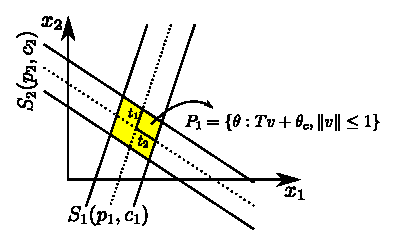
\includegraphics[width=0.92\linewidth]{StripInter}
  \caption{Example of two strips in $\mathbb{R}^{2}$ creating a Parallelotope}
  \label{fig:StripInter}
\end{figure}
%
For simplicity we will restrict the presentation to considering the system \eqref{subeq:Linear_Discrete_system} with $m=1$. The $k^\mathrm{th}$ measurement $y_{m}(k)$ with the bounded measurement error $\epsilon_k \in [-\epsilon_k ,\epsilon_k]$ can be represented as $y_{m}(k) = \ve C^T \ve x(k) + \epsilon_k$. This generates two linear inequalities $(y_{m}(k)-\epsilon_{k} \leq y(k) \leq y_m(k)+\epsilon_k)$, where $y(k)$ is the output predicted by the model, which assumes $\epsilon_k=0,\forall k$. The resulting measurement set $\mathcal{S}_k$ can be represented as
\begin{align}
 \label{eq:Strip_measurement}
 \ve{\mathcal{S}_{k} := \{ x,|C^{T}x - y_m(k)| \leq \epsilon_k \}},
\end{align}
The strip $k$ is almost of the form of \ref{eq:stripdef}; it is only left to be normalized.
\begin{align}
 \label{eq:Strip}
 \mathcal{S}(\ve p_k,c_k):= \left\{\ve\theta\,|\, \left|\ve p_k^T \ve\theta - c_k \right| \leq 1\right\}.
\end{align}
Now the vector $\ve p_k$ is a normal vector to the hyperplanes that bound the strip. The magnitude of $\ve p_k$ determines the width of the strip. The scalar $c_k$ stands for a shift of the strip from the origin.

In addition, it is clear that the intersection of $n$ non parallel strips of the form \ref{eq:Strip} contains the true value of the states and represent a parallelotope (accordingly to \ref{fig:StripInter}. This is,
\begin{align}
 \label{eq:Convex-Polytope}
\textstyle\bigcap_{k=1}^n \mathcal{S}(\ve p_k,c_k )\equiv P(T,\theta_c)
\\
\{\ve\theta:\|\ve P \ve\theta - c \|_{\infty} \leq 1 \} \equiv P(T,\theta_c)
\\
\{ \ve\theta\, |\, \|\ve P(\ve \theta-\ve \theta_c )\|_\infty \leq 1 \} \equiv P(T,\theta_c) 
\end{align}
where $\theta_c=P^{-1}c,$ and P is full rank, obviously, due the condition of non parallel strips. To get the generator form of the parallelotope is needed to make two substitutions. $v:=P(\theta -\theta_{c})$ and $T:=P^{-1}$. 
\begin{align}
 \label{eq:Parallelotope_Grep} 
 \{\ve \theta\,|\, \ve \theta=\ve\theta_c + \ve T \ve v, \|\ve v\|_\infty \leq 1 \} \equiv P(T,\theta_c)
\end{align}
where the columns of $\ve T:=(\ve t_1, \ldots, \ve t_n)$ are called generators. These columns $\ve t_i$ represent directions from the parallelotope center to its faces.
\subsection{Recursive Optimal Parallelotopic Outbounding}
\label{subsec:ROPO}
There are many ways in which parallelotopic approximation can be exploited in set-membership identification. In this paper we consider the sequential approximation problem under a feedback-MPC approach. The ROPO algorithm solves how to find a parallelotope from the intersection of $n+1$ strips. This is, given a parallelotope at the time $k+1$ ( $n$ strips) which contain the real value of the system and a strip who got the real value too at the time $k+1$. The bounding polytope is then given by
\begin{align}
 \label{eq:Prediction_measurement_intersection}
 \mathcal{V}_{k+1} := \mathcal{P}_{k+1|k} \textstyle\bigcap \mathcal{S}_0 =
 \textstyle \bigcap_{\substack{i=0}}^n \mathcal{S}_i,
\end{align}
where $\mathcal{P}_{k+1|k}$ is the parallelotope predicted based on $\mathcal{P}_{k}$ and the system model~\eqref{subeq:Linear_Discrete_system_state} as
\begin{align}
 \ve\theta_{c,k+1} = \ve A\ve\theta_{c,k} + \ve B \ve u_k,
 \quad \ve T_{k+1} = \ve A\ve T_{k}.
\end{align}
The algorithm assumes that the direction vectors $\ve t_i$ of the parallelotope $\mathcal{P}_{k+1|k}$ are such that $\ve p_0^T\ve t_i \geq 0,\ \forall i = \{1, \ldots, n\}$, which represents the projections of the generators $\ve t_i$ on the vector $\ve p_0$.This assumption amounts to fixing appropriate positive directions along the axes of the parallelotope and requires replacing $t_i$ by $-t_{i}$ in the matrix $T$ for those indexes for which the inequality above is not satisfied. Scalars ${\epsilon}_0^+ $ and ${\epsilon}_0^-$ are introduced
\begin{align} 
 {\epsilon}_0^\pm := ( \ve p_0^T \ve\theta_c -c_0 )
 \pm \textstyle\sum_{i=1}^n \ve p_0^T \ve t_i.
%
\end{align}
\begin{figure*}
  \centering
  \includegraphics[width=0.95\linewidth]{"ROPO"}
  \caption{Illustration of the ROPO algorithm in two-dimensional state space.}
  \label{fig:ropo_alg}
\end{figure*}
%
The ROPO algorithm identifies the minimal volume parallelotope outbounding $\mathcal{V}_{k+1}$ in three steps.
\subsubsection{Step 1: Tightening the measurement strip $\mathcal{S}_0$}
As the measurement strip may not completely overlap with $\mathcal{P}_{k+1|k}$ (as shown in Fig.~\ref{fig:ropo_alg}), a new strip $\bar{\mathcal{S}}_0(\bar{\ve p}_0,\bar{c}_0)$ is defined
 \begin{align}
 \bar{\ve p}_0 = \frac{2}{r_0^+ + r_0^-} \ve p_0, \ \
 \bar{c}_0 = \frac{2}{r_0^+ + r_0^-} \left( c_0 + \frac{r_0^+ - r_0^-}{2} \right),
 \end{align}
where $r_0^+ := \min(1,{\epsilon}_0^+)$ and $r_0^- := \min(1,-{\epsilon}_0^-)$.

\subsubsection{Step 2: Reducing the parallelotope $\mathcal{P}_{k+1|k}$}
This reduced parallelotope will play an important role to guarantee feasibility inside the optimization problem. In this paper, it is referred as inner parallelotope. To reduce the non-overlapping volume of $\mathcal{P}_{k+1|k}$, the vectors $\ve t_i$ can be scaled (see Fig.~\ref{fig:ropo_alg}) so the inner parallelotope $\bar{\mathcal{P}}_{k+1|k} := \mathcal P (\bar{T},\bar{\theta}_c)$ is found according to (for $i\in\{1,\ldots,n\}$). 
\begin{align} 
 \bar{\ve t}_i := \frac{r_i^+ + r_i^-}{2} \ve t_i, \quad
 \bar{\ve\theta}_c := \ve\theta_c + {\textstyle\sum_{i=1}^{n}} \frac{r_i^+ - r_i^-}{2} \ve t_i,
\end{align}
\begin{align}
\text{with } r_i^\pm := \begin{cases}
         \min \left(1,\frac{1\mp{\epsilon}_0^\mp}{\ve p_0^T \ve t_i}-1 \right),
          & \textrm{if} \ \ve p_0^T \ve t_i \neq 0,\\
         1, & \textrm{if} \ \ve p_0^T \ve t_i = 0.
         \end{cases}  
\end{align}

\subsubsection{Step 3: Selecting the minimal volume parallelotope $\mathcal{P}_{k+1}$}
\label{SelectingP} As there are $n+1$ strips defining the intersection $\bar{\mathcal{P}}_{k+1|k} \cap \bar{\mathcal{S}}_0$, there are $n+1$ possible parallelotopes for outbounding the intersection. Unless, the measurement strip is a parallel of any strips of the parallelotope($\mathcal{P}_{k+1}$) in which case there is only $n$ possible parallelotope. See Fig.~\ref{fig:ropo_alg} for $n=2$.
The minimum-volume parallelotope is selected by removing the strip $\mathcal S_{i^\ast}$ with the largest projection on $\ve p_0$.
\begin{align} \label{eq:ROPO_criteria}
  i^* := \arg \max_{j\in\{0,1,\ldots,n\}} \bar{\ve p}_0^T \bar{\ve t}_j, \qquad \textrm{with} \ \bar{\ve t}_0 := \bar{\ve p}_0/|\bar{\ve p}_0|^2.
\end{align}
The resulting outbounding parallelotope is given by
\begin{subequations}\label{eq:ROPO_Step3}
\begin{align}
 \mathcal{P}_{k+1} &:= \begin{cases}
                           \bar{\mathcal{P}}_{k+1|k} (\bar{\ve T},\bar{\ve\theta}_c),
                           & \text{if } i^* := 0,\\
                          \mathcal{P}^* (\ve T^*,\ve\theta_c^*), & \text{otherwise},
                          \end{cases}\\
\label{subeq:18b}
\text{where }\quad \ve\theta_c^* &:= \bar{\ve\theta}_c + \frac{1}{\bar{\ve p}_0^T
 \bar{\ve t}_{i^*}} \bar{\ve t}_{i^*} \left(\bar{c}_0 - \bar{\ve p}_0^T
 \bar{\ve \theta}_c \right),\\
 \label{subeq:18c}
\ve t_i^* &= \begin{cases}
               \bar{\ve t}_i - \frac{\bar{\ve p}_0^T \bar{\ve t}_i}
               {\bar{\ve p}_0^T \bar{\ve t}_{i^*}} \bar{\ve t}_{i^*},
               &\text{if } i \neq i^*,\\
               \frac{1}{\bar{\ve p}_0^T \bar{\ve t}_{i^*}} \bar{\ve t}_{i^*},
               & \text{otherwise}.
               \end{cases}
\end{align}
\end{subequations}

\subsection{Measurement-prioritized ROPO algorithm (ROPOm)}
\label{subsec:ROPOm}
In \citep{udit2018} are presented different alternatives of ROPO. One of them is based on the strips measurement and it is shown below.
The measurement prioritized parallelotopic bounding algorithm (ROPOm) is based on the same principle of ROPO, but, the way of how ROPOm selects the resulting parallelotope is a sightly different. $\bar{\mathcal{S}}_0$ is incorporated in the procedure~\eqref{eq:ROPO_criteria}--\eqref{eq:ROPO_Step3} as
\begin{align} \label{eq:ROPOm_vector}
 i^* := \arg \max_{j\in\{1,\ldots,n\}} \bar{\ve p}_0^T \bar{\ve t}_j, \qquad \textrm{with} \ \bar{\ve t}_0 := \bar{\ve p}_0/|\bar{\ve p}_0|^2.
\end{align}
\begin{align}\label{subeq:ROPOm_criteria}
\mathcal{P}_{k+1} := \begin{cases}
                          \bar{\mathcal{P}}_{k+1|k} (\bar{\ve T}, \bar{\ve \theta}_c),& \textrm{if}\ \textstyle\sum_{j=1}^n \bar{\ve p}_0^T \bar{\ve t}_j \leq \bar{\ve p}_0^T \bar{\ve t}_0,\\
                          \mathcal{P}^* (\ve T^*, \ve \theta_c^*),& \textrm{if}\ \textstyle\sum_{j=1}^n \bar{\ve p}_0^T \bar{\ve t}_j > \bar{\ve p}_0^T \bar{\ve t}_0,
                         \end{cases}
\end{align}
where $\ve t_i^*$ and $\ve\theta_c^*$ are defined as in~\eqref{eq:ROPO_Step3}. This leads to the outbounding parallelotope $\mathcal{P}_{k+1}$ lying within the measurement strip. In the ROPOm algorithm, the sum of projections $\sum_{\substack{j=1}}^n \bar{\ve p}_0^T\bar{\ve t}_j$ is compared with the width of strip $\bar{\mathcal{S}}_0$. If the sum is greater than the width \eqref{subeq:ROPOm_criteria}, then the minimal volume parallelotope $\mathcal{P}^*$ within the reduced measurement strip $\bar{\mathcal{S}}_0$ is selected.
\subsection{ROPO Extreme algorithm (ROPOe)}
In case there is not a parallel strip with the parallelotope, there will be $n+1$ possible parallelotope that contains the true values of the system. In this case, it is decided to take two of all possible ones. One will get the minimum distance between its center, $\theta_{c}$, and the measurement output, $y_{m}$, and it is going to be denoted as $P_{m}(T_{m},\theta_m)$. Meanwhile, the another will get the maximum distance and it will denote like $P_{M}(T_{M},\theta_M)$. On the other hand, it is selected another parallelotope, $P(T,\theta_{c}$. This time based on the parallelotope with the minimum volume contained in the strip. This is obtained by discarding the strip in \ref{eq:ROPO_criteria}, therefore, it is only used the equations \ref{subeq:18b} \ref{subeq:18c}. After getting all parallelotopes, these are intersected finding the predictive parallelotope that the MPC is going to use. All parallelotopes must be propagate using \ref{eq:Prediction_measurement_intersection} and with the finality of avoiding unfeasible solution, it is very important reduce $P_{m}(T_{m},\theta_m)$ and $P_{M}(T_{M},\theta_M)$. A detail description of the method is in the Algorithm \ref{alg:ROPOe}.
\begin{algorithm}
\caption{ROPO Extreme algorithm}
\label{alg:ROPOe}
\textbf{Input:} $T,T_{M},T_{m}, \theta_c,\theta_{M},\theta_{m}, S_{0}(p,c)$,\\
\textbf{Initialization:} $T_{M}:=T_{m}:=T$ $\theta_{M}=\theta_c,\theta_{m}=\theta_c$\\
\textbf{Main Loop:}After the first iteration
\begin{enumerate}
\label{en:paramb}
\item Reduce Extreme Parallelotopes.It is recommend to use ROPO or the inner parallelotope, together to the strip.
\item Find the distances. This is $Em=C*\theta_{m}-y_{m}$ and $EM=C*\theta_{M}-y_{m}$
\item Find the parallelotope on the strip
\item Find the distances. This is $E=C*\theta_{c}-y_{m}$
\item Check distance. 
\begin{enumerate}
	\item \textbf{if} $E>EM$ \textbf{then} update $P_{M}$
	\item \textbf{if} $E<Em$ \textbf{then} update $P_{m}$	
\end{enumerate}
\item Intersect $P(T,\theta_c) = P_{M}(T_{M},\theta_M) \cap P_{m}(T_{m},\theta_m)\cap P(T,\theta_c)$
\begin{enumerate}
\item decompose one parallelotope in strips. Use ROPO and repeat with the next parallelotope. 
\end{enumerate}
\end{enumerate}
\textbf{Output:} $P(T,\theta_c)$
\end{algorithm}
\label{subsec:ROPOm}
\subsection{ROPO algorithm Minimum Cost(ROPOmc)}
This method consist in take the best parallelotope based on the cost function of one optimization problem. The algorithm could be resume in
\begin{enumerate}
\item [a)]Select 2 possible parallelotopes. For this task
\begin{enumerate}
\item [a.1)]Apply ROPO algorithm. Once it is known which is the minimum.
\item [a.2)]Delete that column and apply (\ref{eq:ROPO_criteria}) again.  
\end{enumerate}
\item [b)] Find the optimal solution for both parallelotope. Keep the cost of each one.
\item [c)] Compare the cost each one and select the minimum cost.
\end{enumerate} 
\label{subsec:ROPOm}
% ======================================================================
\section{MPC using set-membership approach}
\label{sec:MPC}
Several robust MPC strategies exist to deal with the uncertainties present in the plant model~\citep{Mayne2014}. We use the well-known min-max MPC~\citep{Bemporad1999} approach in this paper, which minimizes the objective function for the uncertainty realization which has the worst (or maximum) cost. One of the major disadvantages of the robust MPC strategies is the conservativeness introduced by these approaches in the presence of large uncertainties. The conservativeness of such schemes can be lowered by reducing the range of uncertainties present in the plant model, \eg by state estimation.

\citep{Garulli1997} combined the state estimation using the set-membership technique with MPC. The overall control strategy for a system in the presence of uncertain initial conditions $\mathcal{P}_{0}$ and measurement error $v_{k+1}$ is shown in Fig.~\ref{fig_mpc_smt}. In the first time step, the min-max MPC is solved considering all initial conditions in $\mathcal{P}_{0}$ and the first control input is applied to the plant. Once the plant measurements are available, $\mathcal{P}_{k+1}$ is computed based on the choice of the set-membership technique discussed in section~\ref{sec:estim}, and the MPC is re-solved using $\mathcal{P}_{k+1}$ as the initial conditions. This procedure is repeated until the end.

\begin{figure}
 \centering
 \includegraphics[width=0.95\linewidth]{"MPC Diagram"}
\caption{MPC using set-membership technique.}
\label{fig_mpc_smt}
\end{figure}

Given the parallelotope $\mathcal P_{k}\ni\ve x_k$, the min-max MPC~\citep{Bemporad1999} solves the problem
\begin{subequations}\label{eq:minmaxmpc}
\begin{align}
\min_{u_i,\ i\in\mathbb I_i:=\{k,\ldots,N_p+k\}}
\max_{j\in\mathbb I_j} \textstyle\sum_{i=k}^{k+N_p}J(x^j_{i+1},u_i), \label{eq:minmax:obj}
\intertext{s.t. }\label{eq:minmax:cons}
\begin{array}{c}
\forall i\in\mathbb I_i\\ \forall j\in\mathbb I_j
\end{array}
\begin{cases}
\ve x^j_{i+1} = \ve A\ve x^j_i + \ve B\ve u_i, \
\ve x^j_k = \ve\theta_c+\ve T\ve\alpha^j,\\
\ve x^j_{i+1} \in \mathcal{X}, \ \ve u_{i} \in \mathcal{U}, \
\ve C\ve x^j_{i+1} \in \mathcal{Y}_c,
\end{cases}
\end{align}\end{subequations}
where $\mathbb I_j$ is an index set of $\{\ve\alpha\,|\,\|\ve\alpha\|_1=n, \|\ve\alpha\|_\infty\leq1 \}$. The sets and $\mathcal{X}$, $\mathcal{U}$ and $\mathcal{Y}_c$ represent the state, input and output constraints, respectively.

Due to the linearity of the process model, the set of all possible evolutions of the plant along the prediction horizon lies in $\text{co}\{x_{i}^j|j\in\mathbb{I}_j\}$~\citep{Scokaert1988}, where $x^j_{i}$ represents the vertex of $\mathcal P_i, \forall i\in\mathbb I_i$. This property ensures the robustness of the calculated control actions $\ve u_k$. To avoid the bi-level optimization, the problem~\eqref{eq:minmaxmpc} can be transformed using the epigraph reformulation with additional inequality constraints~\citep{Lof2003} as
\begin{subequations}
\begin{align}\label{eq:epigraph_minmax}
 \min_{u_j} & \ \Psi\\
 \text{s.t. } & \textstyle\sum_{i=k}^{k+N_p}J(x^j_{i+1},u_i) \leq \Psi, \quad \forall i\in \mathbb I_i, \forall j\in\mathbb{I}_j,\\
 &\text{\eqref{eq:minmax:cons}}.
\end{align}
\end{subequations}
% ====================================================================
\section{Simulation case study}\label{sec:casstu}
The double integrator system is studied in the context of output-feedback min-max MPC with the presented state-estimation algorithms. The process is given as in~\eqref{subeq:Linear_Discrete_system} with
\begin{align}
\ve A := \begin{bmatrix} 1 & 1 \\ 0 & 1 \end{bmatrix}, \
\ve B := \begin{bmatrix} 0\\ 1 \end{bmatrix},\
\ve C := \begin{bmatrix} 1 & 0 \end{bmatrix},\
\end{align}
with $x_{1} \geq 0$, where the states $x_1$ and $x_2$ represent the position and the velocity of an object, respectively. The input $u$ represents object's acceleration at time $k$. The initial state vector $\ve x_0 := (x_{1,0},x_{2,0})^T$, unknown to both the estimator and the MPC controller, is $(20 , 0)^T$. The measurement matrix $\ve C := [1 \ 0]$ depicts the measurement of the position at a sampling rate of 1 time unit and the uniformly distributed measurement error is constant and given $\epsilon_{k}=1$. Finally, it is assumed that exist constraints in the input control $\sim \mathcal U[-1,1]$.

The objective of the optimization problem is to steer the object to position zero with zero velocity, which is represented by a stage cost of the MPC controller~\eqref{eq:epigraph_minmax} with $\ve Q=\ve I$ and $\ve R=0$. For the problem~\eqref{eq:minmaxmpc}, we choose $N_p = 10$ as the prediction horizon.

The cumulative cost is used as a performance index for comparing the estimation concepts
$PI(k) = \sum_{i=1}^{k}(x(k)^{T}Qx(k))$. The uncertainty in the initial states is assumed to be $\pm 1$. For the simulations, the initial parallelotopic set $\mathcal{P}_0$ is selected such that it includes the true state. The initial parallelotope is represented as
\begin{align}
\mathcal{P}_0 = 
  \begin{bmatrix} \theta_{1c,0} \\ \theta_{2c,0} \end{bmatrix}
  + \begin{bmatrix} 2 & 0\\ 0 & 2 \end{bmatrix}
  \alpha, \quad \|\alpha\|_\infty \leq 1,
\end{align}
The parallelotope center  $\ve\theta_{c,0} = [\theta_{1c,0} \ \theta_{2c,0}]^T$ influences the location of the uncertain set; 10 different initial sets are used for simulations by selecting evenly distributed $\theta_{1c,0} \in [18,22]$ and $\theta_{2c,0} \in [-2,2]$. For comparing the controller performance the cumulative performance is averaged for all these sets. The measurement noise is simulated with the same realization of uniformly distributed random noise.

\subsection{States and Bounds}
They are able to show the effectiveness of tracking the system in the term of the output. In the figure \ref{x1prom} is presented the average $x_{1}$ state for all the realizations. It is clear that ROPOmc holds the best output. ROPOe on the other part, it keeps the second place for reach the reference before the $tantos seconds$. As \ref{udit2018} showed before, the ROPOm is superior to ROPO. For the $x_2$ is the same trend. It is relevant to recall this state is not under constraints. The char about $x_2$ is shown in the figure \ref{x2prom}.
\begin{figure}
  \centering
  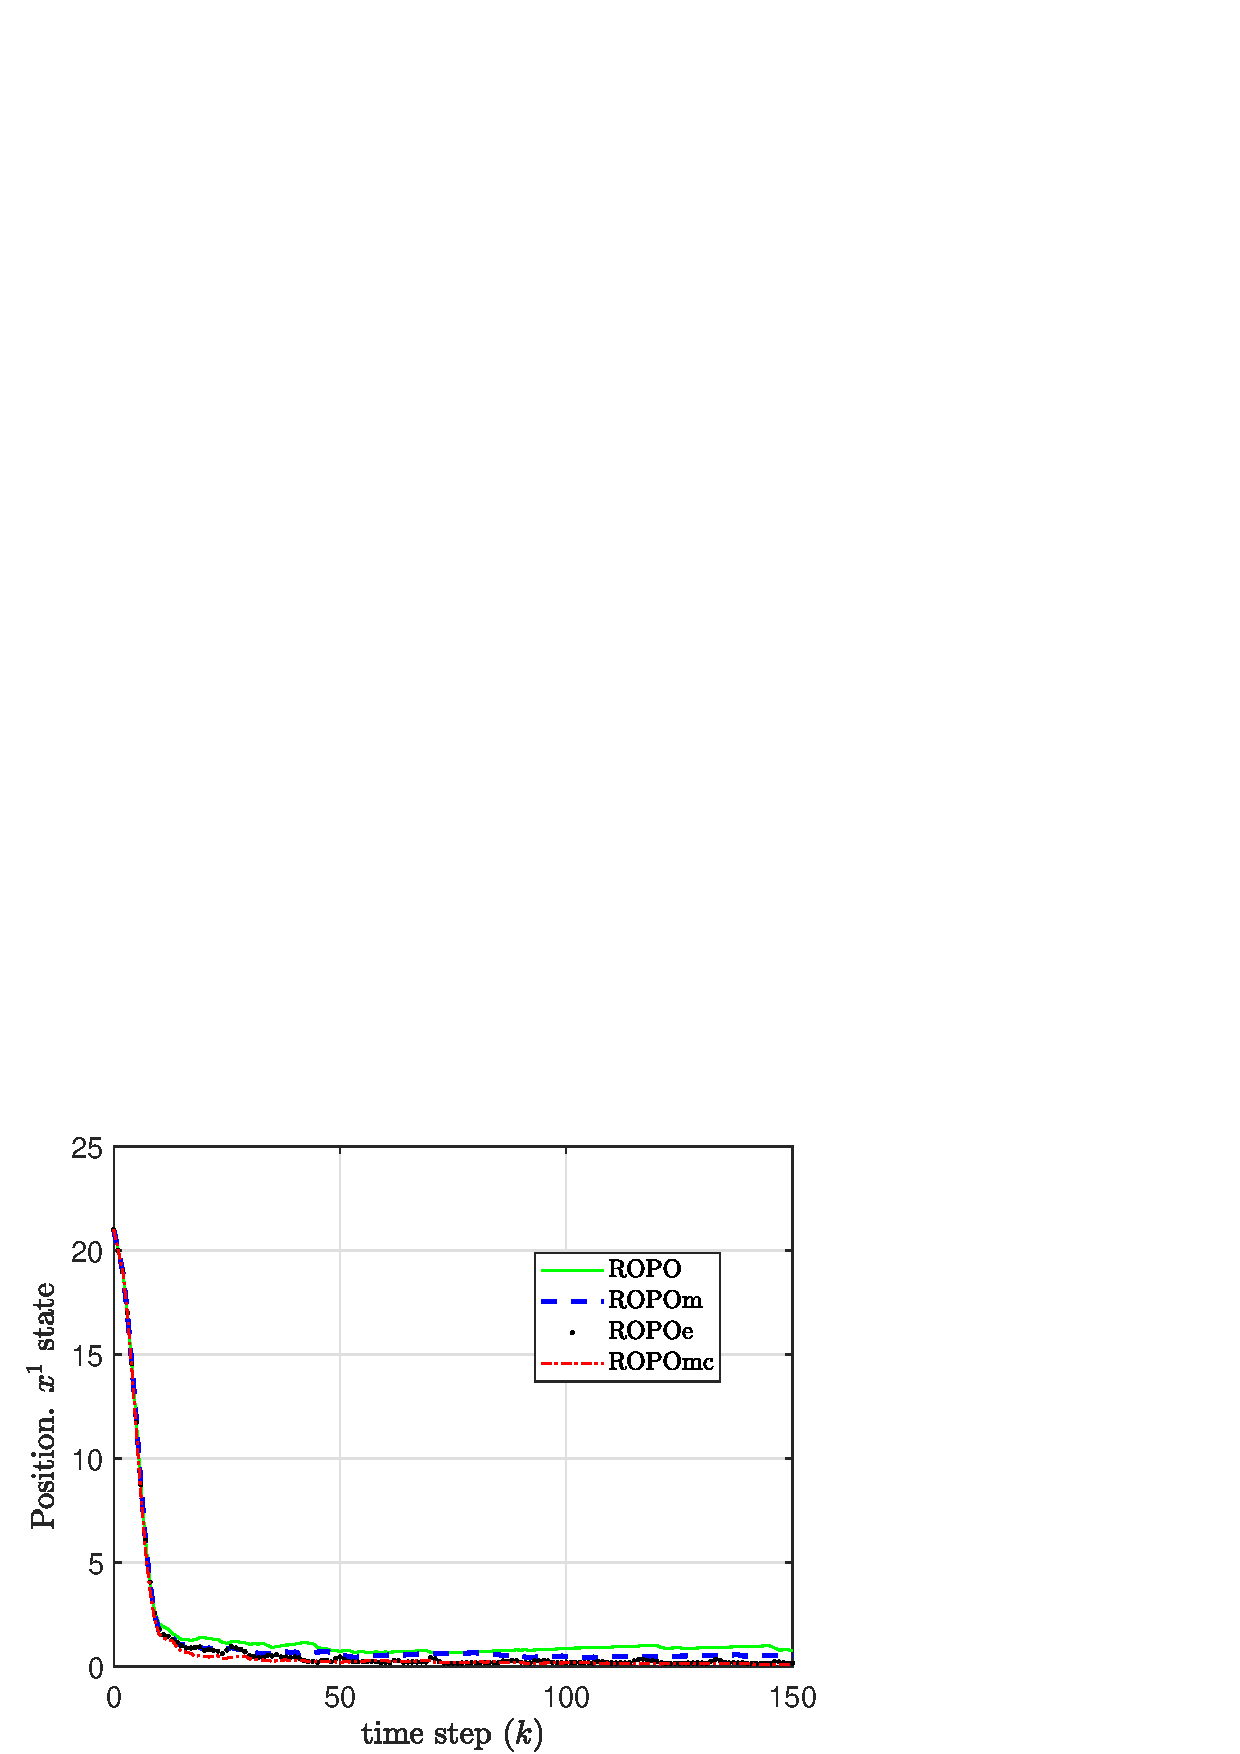
\includegraphics[width=0.95\linewidth]{x1prom}
  \caption{Closed-loop evolution of $x_{1}$ after 10 different realizations. All approaches}
  \label{fig:x1prom}
\end{figure}
\begin{figure}
  \centering
  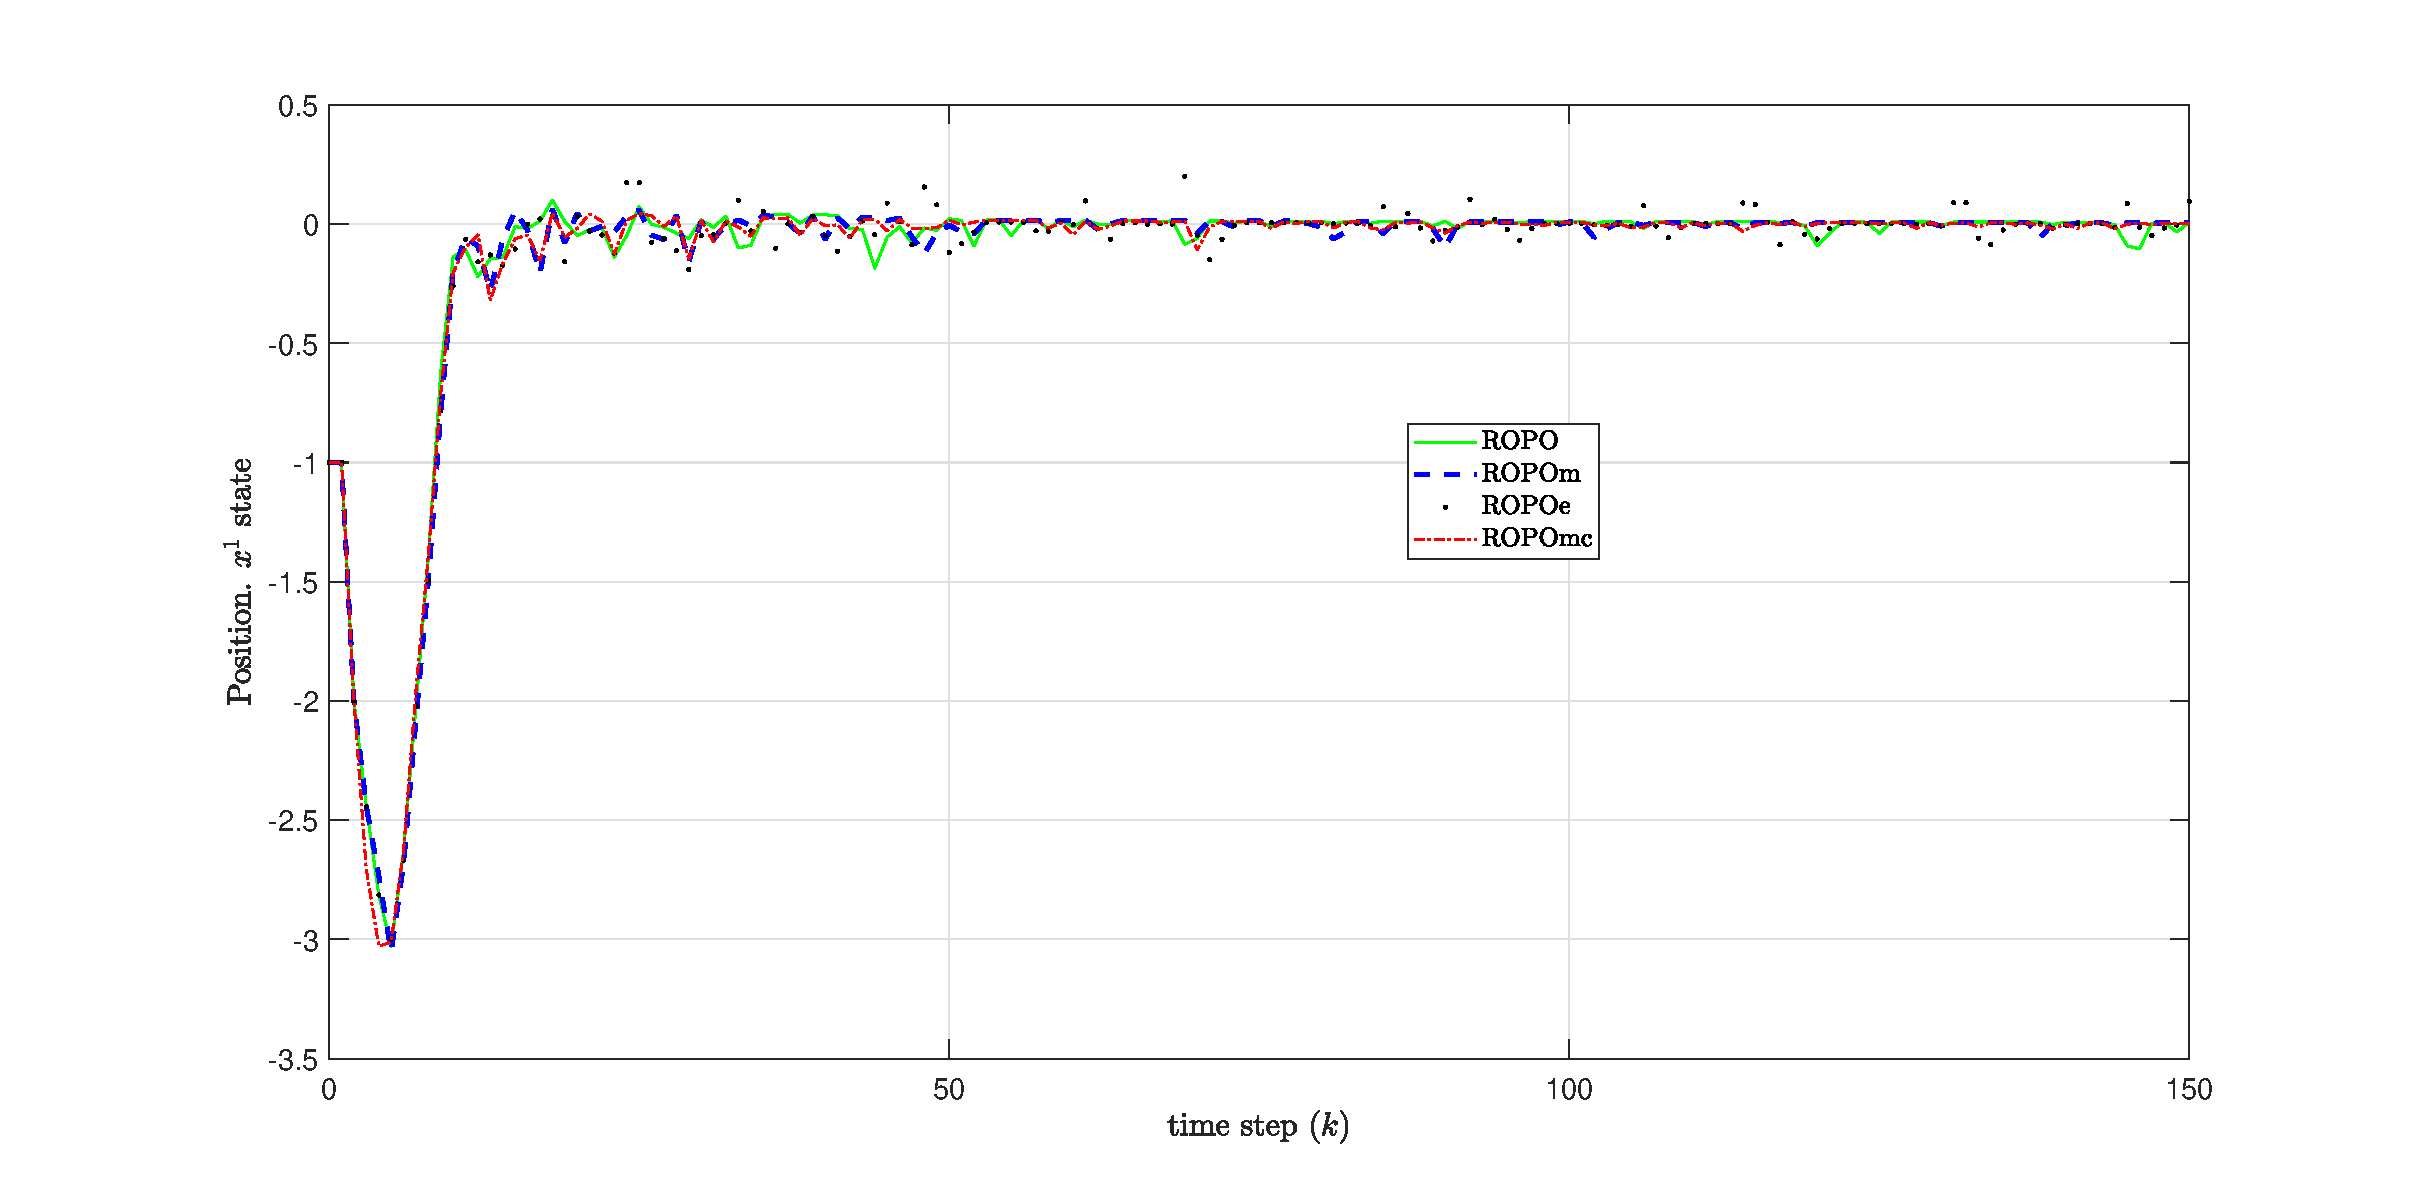
\includegraphics[width=0.95\linewidth]{x2prom}
  \caption{Closed-loop evolution of $x_{2}$ after 10 different realizations. All approaches}
  \label{fig:x2prom}
\end{figure}

The Figure ~\ref{fig:Allx1} shows the average bounds, minimum and maximum of all approaches and realizations.Hence, it does not correspond to any particular case, but enclosure the general tendency. The minimum and maximum values of the state is represented with a unique color for both bounds. On the other hand, the lower bound describes almost the same behavior for the whole different methods. Only in some small cases where the ROPOe exhibits a little hills specially at the beginning. The lower ROPOmc bound is the softest of all.
Furthermore, the higher bound describes very different heights. The minor of all is corresponded to the ROPOmc, follow by the ROPOe and ROPOm and in the last case the well-known ROPO.\\
The MPC method applied here, it take the bounds of the state\\
\begin{figure}
  \centering
  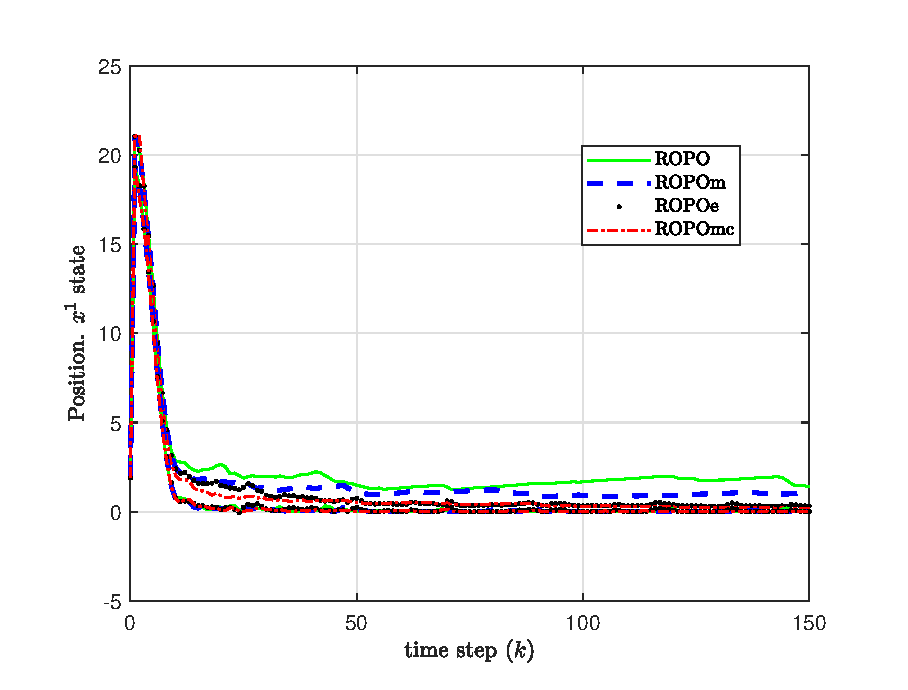
\includegraphics[width=0.95\linewidth]{x1150}
  \caption{Closed-loop evolution of $x_{1}$. All approaches}
  \label{fig:Allx1}
\end{figure}
On the other hand, after 10 different realizations in all methods with the double integrator as the plant. It was obtained the mean and standard deviation(std) for their particular objective functions. In the case of the ROPO algorithm, the average performance was around $2064.5$ with an std of $116.9$. The Ropo measurement algorithm of \citep{udit2018} improve this result in both senses, mean with $2034.8$ and std with $101.9$. In the same way, the new approaches, ROPO extreme and ROPO minimum cost show the same downward tendency. ROPOe for its part got a mean of $2015.1$ and an std of $94.6$ even less than the previous methods. However, the ROPOmc exhibits a mean of $1967.3$ and an std of $49$ the lowest values of all approaches, pushing this like the best technique considering only the objective function as a performance index. A graphical representation of this is shown in the Figure ~\ref{fig:stdApproaches}.
\begin{figure}
  \centering
  \includegraphics*[width=0.95\linewidth]{stdApproaches}
  \caption{State uncertainty sets for ROPO and ROPOc estimation algorithms for $\ve\theta_{c,0} = (21, 2)^T$.}
  \label{fig:stdApproaches}
\end{figure}
\\
\\
\begin{figure}
  \centering
  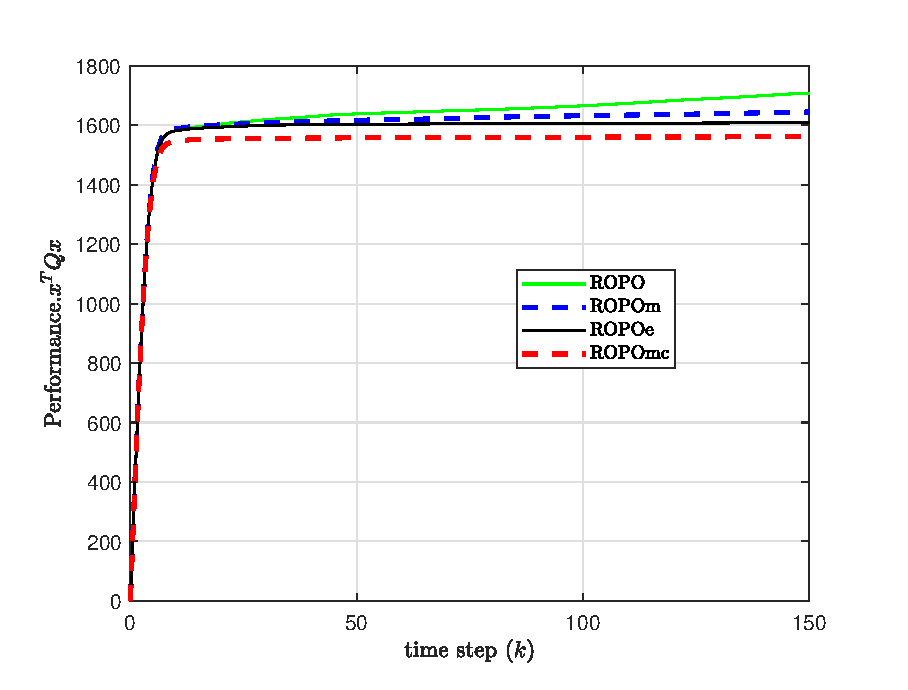
\includegraphics[width=0.8\linewidth]{Performance}
  \caption{Accumulative Performance for all approaches.}
  \label{fig:case_constrained_variable}
\end{figure}
In our computational experience, ROPO, ROPOm and ROPOe exhibit roughly the same CPU time (within 0.001\,s). Even when ROPOe implies to run ROPOm plus the intersection using ROPO, hence this algorithm require more CPU time. However, it is not significantly. On the contrary, ROPOmc algorithm takes much more time (200-fold increase) because it resolve two optimization problem, meanwhile the rest only one. But it is the perfect option for the majority of the case in industry which they tend to be slow dynamics.

%======================================================================
\section{Conclusions}\label{sec:conclu}
In this paper, we combined the robust min-max model predictive control with set-membership state estimation, considering systems with uncertainties in initial conditions under hard input and state constraints. With ten possible realizations in the state set $\mathcal{P}_{k}$, the control action is limited by the realization with active constraint or the maximum cost. Thus for the best robust performance, the set-membership state estimator should not include an outbounding error where the possible states have an active constraint or maximum cost. We proposed alternative estimators, built on the well-known Recursive Optimal Parallelotopic Outbounding (ROPO) algorithm and ROPOm, that prioritize reduction of the outbounding error \wrt the ROPO algorithm Extreme values (ROPOe) and another focus on minimize the cost function of the system subject to a set of constraints(ROPOmc).

In the presented case study the ROPO algorithm was found to cause the worst performance of the resulting control actions. This is mainly due to the selection of minimum volume parallelotope, which may lead to the measurement information being ignored. The ROPOmc estimation algorithm achieved the best performance, because it studies the different possible options,however, it is the worse option in terms of computational cost, thus, it is not a recommended choice for extremely fast dynamic systems. In those case, ROPOe is the best alternative.

The presented extensions of ROPO algorithm may be pave the way for new developments in other advanced estimation algorithms, such as those using zonotopes~\citep{le13book}, ellipsoids~\citep{Filippova1996}, or constrained zonotopes~\citep{Scott2016}. The future work would also focus on applying the developed algorithms in control problem with multiple constraints and in the presence of unmodelled dynamics. An interesting extension would be a combination of the set-membership estimator with scenario-based MPC \citep{ber09}.

\bibliography{ifacconf}             % bib file to produce the bibliography
\end{document}
